\documentclass[pdf,color]{UoBnote}
\usepackage{epstopdf}
\usepackage{float}
\author{Samuel Delacruz\\
				sjd054@bham.ac.uk\\
				1090154}

\shorttitle{}
\title{Computational Modelling of Physical Systems\\Worksheet 2}
\date{\today}
\issue{2}

\begin{document}


\iffalse
	\em{TO DO:}
		Replot graphs with axis labels in GNUplot\\
		Complete Theory sections\\
		Complete programs for 2,6 and 7.\\
		Write up procedure for usage of programs\\
		Create tables of results for 2, 6, 7\\
		Create graphs in GNUPlot for 2, 6, 7 results.\\
		Replot 6 and 7 theory plots with axis labels in GNUplot\\
		Write up comparison - conclusion for 2\\
		Write up conclusions for 6 and 7\\
		Write overall conclusion\\
		Write Introduction to 2, 6, 7\\
		Write overall introduction\\
\fi

\maketitle
\tableofcontents
\listoffigures
\listoftables
\vspace{1cm}\hrule \vspace{1cm}
\newpage

\section{Introduction}
\section{Numerical Integration}
	\subsection{The Trapezium Rule}
		\subsubsection{Theory}
			The trapezium rule can be used as a method of numerically evaluating integrals. It involves splitting a function $f(x)$ into $n$ intervals of separation $h$,
			connected by straight lines. These pieces can be integrated by creating trapzoidal segments and calculating their area, then summing their areas.
			and using their area to approximate the integral of $f(x)$. As $h \rightarrow 0$, the estimated value converges to the exact integral value. The trapezium rule is given as follows:
			
			\begin{equation} \label{eq:trapezium}
				\int\limits_{x_0}^{x_n} f(x) dx \approx \frac{1}{2}h\left[f(x_0) + f(x_n) + 2(f(x_1) + f(x_2) +...+ f(x_{n-1}))\right]
			\end{equation}
			
			Where $h$, the width of the interval is defined by:
			
			\begin{equation} \label{eq:h_def}
				h = \frac{x_n - x_0}{n}
			\end{equation}
			
			Due to the nature of the trapezium rule, there is naturally an error associated with values calculated using it.
			There exists an analytic expression for this error and is given by the following equation $^{\cite{errors_web}}$:
			
			
			\begin{equation} \label{eq:trap_err}
				E_n^T = -\frac{h^2\left(b-a\right)}{12}f''(c_n)
			\end{equation}
			
			Which can be adapted to give the maximum error on the estimated value for the integral of $f(x)$:
			
			\begin{equation} \label{eq:trap_err2}
				\left|E_n^T\right| \leq \frac{h^2\left(b-a\right)}{12}\max_{a \leq x \leq b}\left|f''(x)\right|
			\end{equation}
			
			
			\subsubsection{Procedure}
				
				\begin{figure}[h]
					\centering
						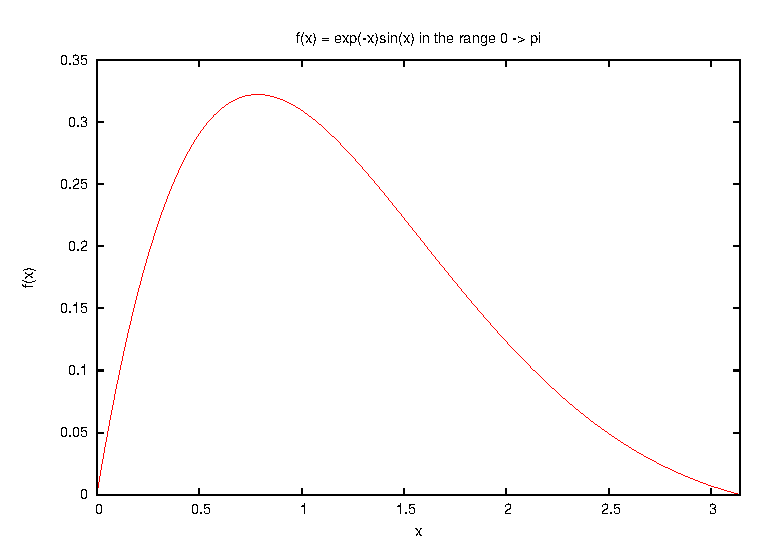
\includegraphics{figures/q2b.eps}
					\caption{Plot of $f(x)$ in the range $[0:\pi]$}
					\label{fig:q2b}
				\end{figure}
				
				In this assignment, the Trapezium rule was used to approximately evaluate a definite integral, given by
				
				\begin{equation}
				\int\limits_0^2 e^{-x}\sin{(x)} dx	
				\end{equation}

				Where $f(x) = e^{-x}\sin{(x)}$ is shown in figure (\ref{fig:q2b})\\				
								
				The integral has an exact value of
				
				\begin{equation}
				\frac{1}{2} - \frac{\sin{2}+\cos{2}}{2e^{-2}}
				\end{equation}
				
				Which is equal to $0.466629662593175$ (15 decimal places).\\							
				\begin{figure}[H]
					\centering
						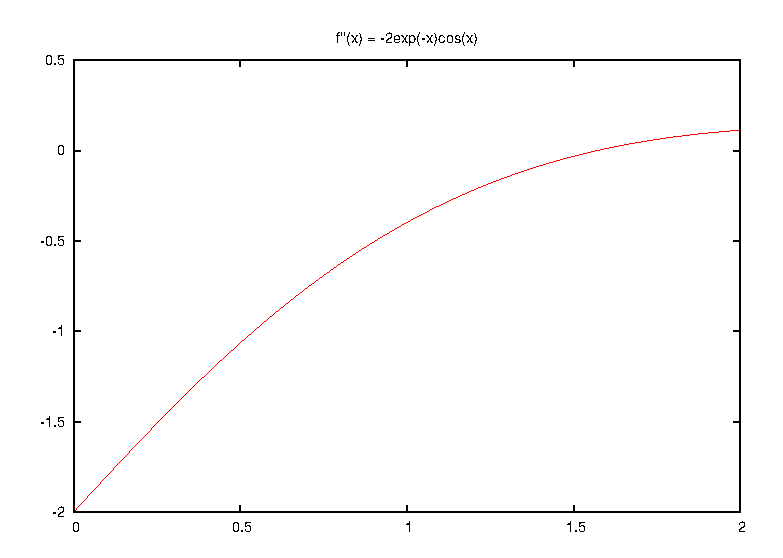
\includegraphics{figures/q2-f2x-trap.eps}
					\caption{Plot of $f''(x)$ in the range $[0:2]$}
					\label{fig:q2-f2x-trap}
				\end{figure}
				
				From figure (\ref{fig:q2-f2x-trap}) it can easily be seen that $f''(x)$ is maximal at $x=2$, within our limits of integration. So in the equation for maximum estimated error, $f''(x=2)$ is used,\\				
				
				A program was written to evaluate the integral which would write a table to a text file showing the value of the integral calculated against the number of subintervals used in the Trapezium method.
				
				The program was written to the source code file ``q2c.cpp", which may be compiled using g++ in the command line.\\\\
				To run the program, use the following format of command line arguments:\\
				\texttt{./q2c.o n-min n-max output-filename}\\
				
				Where n-min is the minimum number of subintervals to test, n-max is the maximum number of subintervals, and output-filename is the file to save output data to.
				\subsubsection{Results}
				
				\begin{figure}[H]
					\centering
						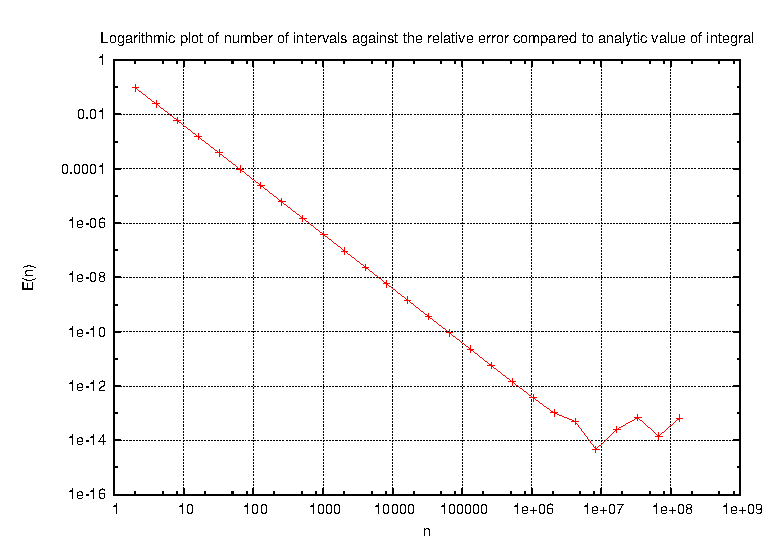
\includegraphics{figures/q2d_labelled.eps}
					\caption{$\log_{10}$ plot of $E(n)$ in the range $n = [1:10^{9}]$ (Trapezium method)}
					\label{fig:q2d}
				\end{figure}
				
				Figure (\ref{fig:q2d}) shows a plot of $\log_{10}$ of the number of intervals used against the $\log_{10}$ of the relative error compared to the exact integral value.\\
				This graph follows the corresponding analytic error predictions (Fig \ref{fig:q2e}) up to a relative error of $\approx 10^{-13}$ where roundoff error provides a fundamental limit to the minimum error attainable by using double precision floating point types.\\
				It is important to note that the Trapezium method is a \emph{very} slow algorithm when approximating integrals of curves, making many calls to $f(x)$ when high accuracy is required. To obtain the previous results, 33554454 calls were made to $f(x)$, which will be shown later to be relatively inefficient compared to other methods.
	
				\begin{figure}[H]
					\centering
						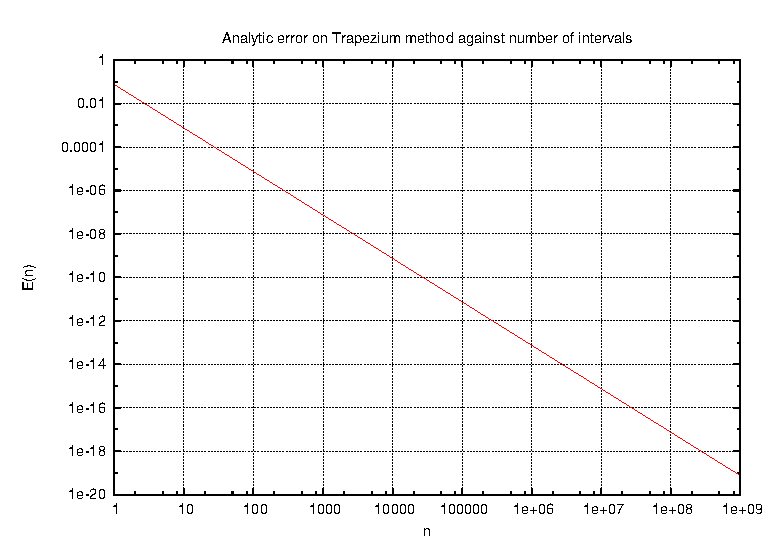
\includegraphics{figures/q2e.eps}
					\caption{$\log_{10}$ plot of $E^T(n)$ in the range $n = [1:10^{9}]$}
					\label{fig:q2e}
				\end{figure}
	
		\subsection{Simpson's Rule}
			\subsubsection{Theory}
				Simpson's rule is another method of computing the value of integrals. Instead of splitting $f(x)$ into straight-line segments as in the trapezium rule, the function is split into a
				series of parabolic segments. This results in a higher level of precision than the trapezium rule, and will be demonstrated in the procedure to follow. The equation for Simpson's rule is given as follows $^{\cite{errors_web}}$:
				
				\begin{equation} \label{simpsons}
					\int\limits_a^b f(x) dx \approx \frac{h}{3}\left[f(x_0) + 4f(x_1) + 2f(x_2) + 4f(x_3) + 2f(x_4) + ... + 2f(x_{n-2}) + 4f(x_{n-1}) +f(x_n)\right]
				\end{equation}
				
				Which may also be written as $^{\cite{simps_wiki}}$:
				
				
				\begin{equation} \label{simpsons_sum}
					\int\limits_a^b f(x) dx \approx \frac{h}{3}\left[f(x_0) + 2 \sum\limits_{j=1}^{(n/2)-1} \left(f(x_{2j})\right) + 4 \sum\limits_{j=1}^{n/2} \left(f(x_{2j-1})\right) + f(x_n) \right]
				\end{equation}
				Where $h$ is given in equation (\ref{eq:h_def})\\\\
				
				There is naturally an error associated with values calculated using Simpson's rule to approximate integrals. 
			There exists an analytic expression for this error and is given by the following equation $^{\cite{errors_web}}$:
			
			
			\begin{equation} \label{eq:simps_err}
				E_n^S = -\frac{h^4\left(b-a\right)}{180}f^{(4)}(c_n)
			\end{equation}
			
			Which can be adapted to give the maximum error on the estimated value for the integral of $f(x)$:
			
			\begin{equation} \label{eq:simps_err2}
				\left|E_n^S\right| \leq \frac{h^4\left(b-a\right)}{180}\max_{a \leq x \leq b}\left|f^{(4)}(x)\right|
			\end{equation}
			
			\begin{figure}[H]
					\centering
						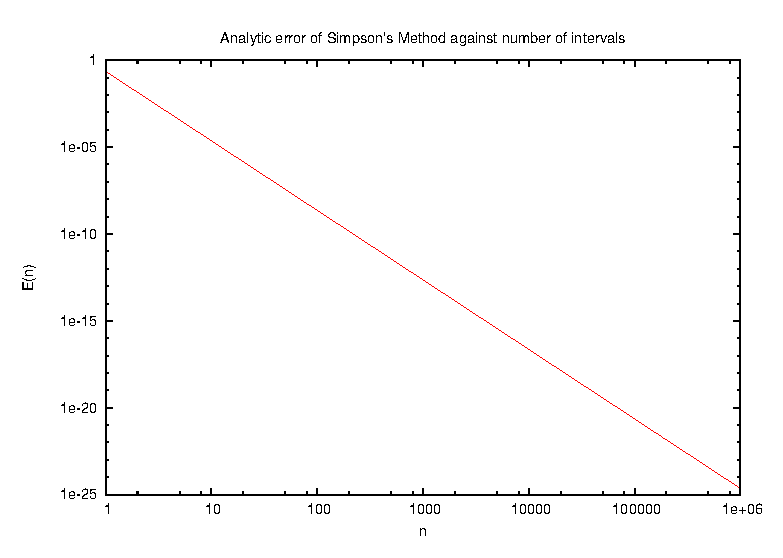
\includegraphics{figures/q2g.eps}
					\caption{$\log_{10}$ plot of $E^S(n)$ in the range $n = [1:10^{6}]$}
					\label{fig:q2g}
				\end{figure}
				
				Through the comparison between the analytic errors of the Trapezium rule (fig \ref{fig:q2e}) and Simpson's rule (fig \ref{fig:q2g}) it is obvious that Simpson's rule converges to a highly accurate result faster than the Trapezium rule.
					
				
			\subsubsection{Procedure}
				
			In this assignment, Simpson's rule was used to approximately evaluate a definite integral, given by
				
				\begin{equation}
				\int\limits_0^2 e^{-x}\sin{x} dx	
				\end{equation}
				
				Where $f(x)$ is shown in figure (\ref{fig:q2b})\\
				
				The integral has an exact value of
				
				\begin{equation}
				\frac{1}{2} - \frac{\sin{2}+\cos{2}}{2e^{-2}}
				\end{equation}
				
				Which is equal to $0.466629662593175$ (15 decimal places).\\				
				\begin{figure}[H]
					\centering
						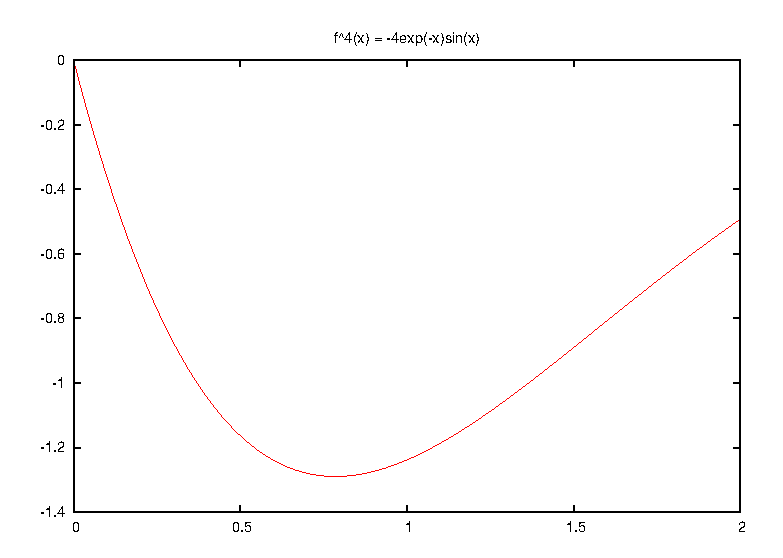
\includegraphics{figures/q2-f4x-simps.eps}
					\caption{Plot of $f^{\left(4\right)}(x)$ in the range $[0:2]$}
					\label{fig:q2-f4x-simps}
				\end{figure}				
				
				From figure (\ref{fig:q2-f4x-simps}) it can be seen that $f^{(4)}(x)$ is minimal at $x=\pi / 4$, within our limits of integration. So in the equation for maximum estimated error, $f''(x=\pi / 4)$ is used.
				
				The program was more sophisticated than the Trapezium rule program, in that the user needs only to supply the desired number of significant figures to calculate with accuracy to, and the output file name.\\
				In order to convert number of desired significant figures of accuracy to numbher of subintervals to use, the following equation was used,
				
				\begin{equation}
				n = \left( \frac{(b-a)^5 \cdot 10^{N_{sf}-1}}{180}\right) 
				\end{equation}
				
				Which is simply a refactoring of the analytical error equation for SImpson's method, and $n$ is the maximum number of subintervals to use.\\
				
				The program was written to the source code file "q2f.cpp", which may be compiled using g++ in the command line.\\
				To run the program, use the following format of command line arguments:\\
				\texttt{./q2f.o sf output-filename}\\
				
				Where ``sf" is the number of significant figures to calculate to, and ``output-filename" is the name of the file to save output data to.
				
				\subsubsection{Results}
				
				\begin{figure}[H]
					\centering
						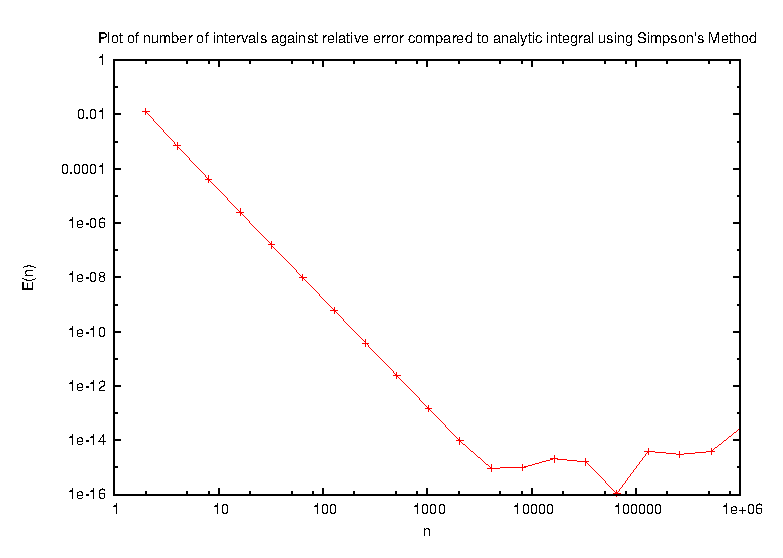
\includegraphics{figures/q2g_computed.eps}
					\caption{$\log_{10}$ plot of $E(n)$ in the range $n = [1:10^{6}]$ (Simpson's method)}
					\label{fig:q2g_computed}
				\end{figure}
				
				Figure (\ref{fig:q2g_computed}) shows a plot of $\log_{10}$ of the number of intervals used in Simpson's method against the $\log_{10}$ of the relative error compared to the exact integral value.\\
				This graph follows the corresponding analytic error predictions up to a relative error of $\approx 10^{-16}$ where roundoff error provides a fundamental limit to the minimum error attainable by using double precision floating point types.\\
				Simpson's method is a faster algorithm than the Trapezium method when approximating integrals of curves, making far fewer calls to $f(x)$ at comparable accuracy. To obtain the previous results, 134217752 calls were made to $f(x)$, however to obtain minimal error at $E(n) \approx 10^{-16}$, 8202 calls were made. For an accuracy of $E(n) \approx 10^{-10}$, 261 calls were made.
				
\section{Numerical Integration with GSL}
	\subsection{GSL QAGS routine for basic numerical integration}
	
		\subsubsection{Procedure}
			Using GSL, a program was written to evaluate the integral previously used for testing the Trapezium and Simpson's methods,
			
			\begin{equation}\label{eq:int1}
				\int\limits_0^2 e^{-x}\sin{(x)} dx	
			\end{equation}
				
			The QAGS routine was chosen as being appropriate for this problem, due to the function being a relatively smooth, non-oscillatory function within the given limits.\\
			A target relative and absolute error of $10^{-10}$ was chosen to be hard coded into the program.\\
			To run the program, use the following format of command line arguments:\\
				\texttt{./q6a.o output-filename}\\
			Where ``output-filename" is the name of the file to be used to save any output data to.
		\subsubsection{Results}
		
		\begin{table}[H]\label{tab:qags-results}
		\centering
		\caption{QAGS Routine Table of Results}
    \begin{tabular}{|l|l|}
    \hline
    result          & 0.466629662593176    \\
    exact result    & 0.466629662593175    \\
    estimated error & 5.18062995384012e-15 \\
    actual error    & 5.55111512312578e-16 \\
    f(x) calls      & 21                   \\
    \hline
    \end{tabular}
\end{table}
			From table (\ref{tab:qags-results}) it can be seen that the QAGS routine was able to calculate the value of the integral to a high precision, at far less function calls to $f(x)$ than either of the two previously used numerical methods.\\
			The QAGS routine is therefore a very efficient and suitable method of integrating simple functions, such as the integral in equation (\ref{eq:int1}).
	\subsection{GSL QAWO routine for functions with oscillatory weight function}
		\subsubsection{Procedure}
			Using GSL, a program was written to evaluate a new integral,
			
			\begin{equation}\label{eq:int2}
				\int\limits_0^{2\pi}x\sin{(30x)}\cos{(x)} dx	
			\end{equation}
			Which has an exact value of $-60\pi/899$
			\begin{figure}[H]
					\centering
						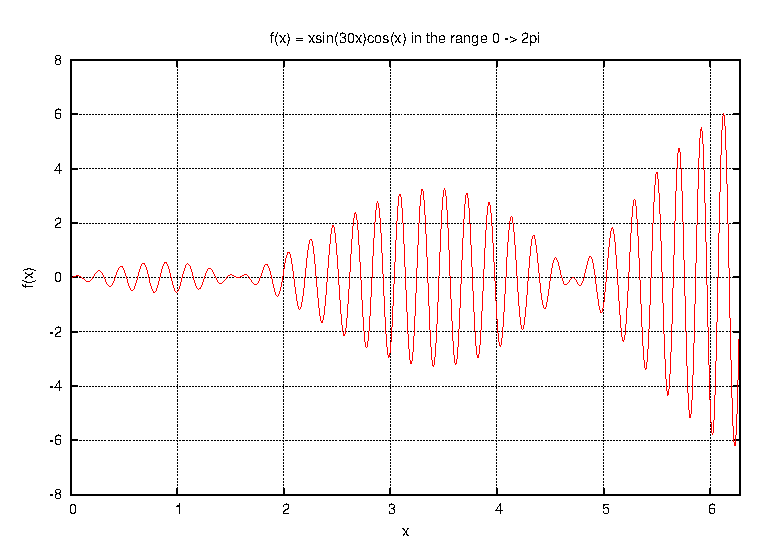
\includegraphics{figures/q7b_labelled.eps}
					\caption{Plot of $f(x)$ in the range $[0:2\pi]$}
					\label{fig:q7b}
				\end{figure}
				This function is one which aught to cause computers reasonable difficulty in calculating to any accuracy, given the oscillatory nature of the function. The trapezium and Simpson's methods would both struggle with this problem, because splitting the function into constituent segments does not make logical sense, unless the segments are much smaller than the $\sin(30x)$ terms.\\
			The QAWO routine was chosen as being appropriate for this problem, due to the function being of the form:
			\begin{equation}
			\int\limits_a^b f(x)\sin(\omega x + \phi) dx
			\end{equation}
			Where in this case, $f(x) = x\cos(x)$, and $\sin(\omega x +\phi) = \sin(30x + 0)$.\\
			The QAWO routine is described in the GSL manual as being more efficient than other routines, such as QAGS, at evaluating integrals of this form.\\
			A target relative and absolute error of $10^{-10}$ was chosen to be hard coded into the program.\\
			To run the program, use the following format of command line arguments:\\
				\texttt{./q7\textunderscore qawo.o output-filename}\\
			Where ``output-filename" is the name of the file to be used to save any output data to.
			
			\subsubsection{Results}
			
			\begin{table}[H]\label{tab:qawo-results}
		\centering
		\caption{QAWO Routine Table of Results}
    \begin{tabular}{|l|l|}
    \hline
    result          & -0.209672479661165    \\
    exact result    & -0.209672479661165    \\
    estimated error & 6.22148543332591e-12 \\
    actual error    & -2.77555756156289e-17 \\
    f(x) calls      & 75                   \\
    \hline
    \end{tabular}
\end{table}			
		
		From table (\ref{tab:qawo-results}) it can be seen that the QAWO routine was able to calculate the value of the integral to a very high precision, at just 75 function calls to $f(x)$.\\
			This is a very satisfactory result, given that the very simple function evaluated in the trapezium and Simpson's methods yielded far more function calls than this vastly more complicated function.\\
			
\section{Appendices}

	\subsection{Tables of Data}
		\subsubsection{Trapezium Rule Approximation Data}
			\begin{table}[H]
			\centering
			\caption{Trapezium Rule Approximation Data}
    \begin{tabular}{|l|l|l|}
        \hline
		Intervals (n) & Approximation (I) & Relative Error (E)\\
		\hline
        2.000000000000000e+00 & 3.710898880560006e-01 & 9.553977453717444e-02 \\
        4.000000000000000e+00 & 4.422236961884555e-01 & 2.440596640471954e-02 \\ 
        8.000000000000000e+00 & 4.604972261865506e-01 & 6.132436406624364e-03 \\ 
        1.600000000000000e+01 & 4.650946458672943e-01 & 1.535016725880689e-03 \\ 
        3.200000000000000e+01 & 4.662457896022591e-01 & 3.838729909159122e-04 \\ 
        6.400000000000000e+01 & 4.665336869263886e-01 & 9.597566678637426e-05 \\ 
        1.280000000000000e+02 & 4.666056682128897e-01 & 2.399438028533041e-05 \\ 
        2.560000000000000e+02 & 4.666236639691317e-01 & 5.998624043324075e-06 \\ 
        5.120000000000000e+02 & 4.666281629353536e-01 & 1.499657821424361e-06 \\ 
        1.024000000000000e+03 & 4.666292876786068e-01 & 3.749145682241384e-07 \\ 
        2.048000000000000e+03 & 4.666295688645267e-01 & 9.372864834267247e-08 \\ 
        4.096000000000000e+03 & 4.666296391610124e-01 & 2.343216259914627e-08 \\ 
        8.192000000000000e+03 & 4.666296567351357e-01 & 5.858039275885574e-09 \\ 
        1.638400000000000e+04 & 4.666296611286658e-01 & 1.464509236104306e-09 \\ 
        3.276800000000000e+04 & 4.666296622270488e-01 & 3.661261849252639e-10 \\ 
        6.553600000000000e+04 & 4.666296625016473e-01 & 9.152767432851761e-11 \\ 
        1.310720000000000e+05 & 4.666296625702892e-01 & 2.288580436271559e-11 \\ 
        2.621440000000000e+05 & 4.666296625874499e-01 & 5.725142582235776e-12 \\ 
        5.242880000000000e+05 & 4.666296625917487e-01 & 1.426359030887170e-12 \\ 
        1.048576000000000e+06 & 4.666296625928048e-01 & 3.702038675612584e-13 \\ 
        2.097152000000000e+06 & 4.666296625930729e-01 & 1.020850071142831e-13 \\ 
        4.194304000000000e+06 & 4.666296625931254e-01 & 4.957145804951324e-14 \\ 
        8.388608000000000e+06 & 4.666296625931709e-01 & 4.107825191113079e-15 \\ 
        1.677721600000000e+07 & 4.666296625931502e-01 & 2.481348460037225e-14 \\
        \hline
    \end{tabular}
\end{table}

		\subsubsection{Simpson's Rule Approximation Data}
			\begin{table}[H]
			\centering
			\caption{Simpson's Rule Approximation Data}
    \begin{tabular}{|l|l|l|}
        \hline
		Intervals (n) & Approximation (I) & Relative Error (E)\\
		\hline
        2.000000000000000e+00 & 4.537665091394085e-01 & 1.286315345376704e-02 \\ 
        4.000000000000000e+00 & 4.659349655659404e-01 & 6.946970272351249e-04 \\ 
        8.000000000000000e+00 & 4.665884028525825e-01 & 4.125974059310256e-05 \\ 
        1.600000000000000e+01 & 4.666271190942090e-01 & 2.543498966611768e-06 \\ 
        3.200000000000000e+01 & 4.666295041805804e-01 & 1.584125951525905e-07 \\ 
        6.400000000000000e+01 & 4.666296527010985e-01 & 9.892077046380621e-09 \\ 
        1.280000000000000e+02 & 4.666296619750568e-01 & 6.181187228726515e-10 \\ 
        2.560000000000000e+02 & 4.666296625545451e-01 & 3.863048769758848e-11 \\ 
        5.120000000000000e+02 & 4.666296625907614e-01 & 2.414124455896172e-12 \\ 
        1.024000000000000e+03 & 4.666296625930244e-01 & 1.511568648027151e-13 \\ 
        2.048000000000000e+03 & 4.666296625931659e-01 & 9.658940314238862e-15 \\ 
        4.096000000000000e+03 & 4.666296625931746e-01 & 9.436895709313831e-16 \\ 
        8.192000000000000e+03 & 4.666296625931766e-01 & 9.992007221626409e-16 \\ 
        1.638400000000000e+04 & 4.666296625931735e-01 & 2.109423746787797e-15 \\ 
        3.276800000000000e+04 & 4.666296625931772e-01 & 1.609823385706477e-15 \\ 
        6.553600000000000e+04 & 4.666296625931755e-01 & 1.110223024625157e-16 \\ 
        1.310720000000000e+05 & 4.666296625931716e-01 & 3.941291737419306e-15 \\ 
        2.621440000000000e+05 & 4.666296625931725e-01 & 3.053113317719180e-15 \\ 
        5.242880000000000e+05 & 4.666296625931717e-01 & 3.885780586188048e-15 \\ 
        1.048576000000000e+06 & 4.666296625931431e-01 & 3.247402347028583e-14 \\ 
        2.097152000000000e+06 & 4.666296625931546e-01 & 2.098321516541546e-14 \\ 
        4.194304000000000e+06 & 4.666296625931952e-01 & 1.965094753586527e-14 \\ 
        8.388608000000000e+06 & 4.666296625930849e-01 & 9.064970996064403e-14 \\ 
        1.677721600000000e+07 & 4.666296625931530e-01 & 2.253752739989068e-14 \\ 
        3.355443200000000e+07 & 4.666296625931158e-01 & 5.978550987606468e-14 \\ 
        6.710886400000000e+07 & 4.666296625932169e-01 & 4.135580766728708e-14 \\
        \hline
    \end{tabular}
\end{table}

\begin{thebibliography}{breitestes Label}
	\bibitem{errors_web} Kendall E. Atkinson\\{\em http://homepage.math.uiowa.edu/\textasciitilde{}atkinson/ftp/ENA\_Materials/Overheads/sec\_5-2.pdf}\\Accessed at 01-11-2013\\
	\bibitem{simps_wiki} Wikipedia.org\\{\em http://en.wikipedia.org/wiki/Simpson's\_rule\#Composite\_Simpson.27s\_rule}\\Accessed at 01-11-2013
\end{thebibliography}

\end{document}
